\documentclass[11pt,a4paper]{article}

\usepackage[T1]{fontenc}
\usepackage[utf8]{inputenc}
\usepackage{lmodern}
\usepackage[margin=2.3cm,top=2.2cm,bottom=2.4cm]{geometry}
\usepackage{microtype}
\usepackage{amsmath,amssymb}
\usepackage{booktabs}
\usepackage{tabularx}
\usepackage{graphicx}
\usepackage[table]{xcolor}
\usepackage{tikz}
\usetikzlibrary{positioning,arrows.meta,fit,calc}
\usepackage[font=small,labelfont=bf,labelsep=period]{caption}
\usepackage[numbers,sort&compress]{natbib}
\usepackage{enumitem}
\usepackage{fancyhdr}
\usepackage{titlesec}
\usepackage[hidelinks]{hyperref}

\definecolor{bacai}{HTML}{0A7A5C}
\definecolor{ink}{HTML}{1B2830}
\definecolor{muted}{HTML}{5A6A74}
\definecolor{rule}{HTML}{C9D3D0}

\hypersetup{colorlinks=true,linkcolor=bacai,citecolor=bacai,urlcolor=bacai,
  pdftitle={Baseline AI: Explainable Machine Learning for Hourly Building Energy Forecasting, Waste Detection and Savings Verification},
  pdfauthor={Abdelouahab KRIM},
  pdfsubject={Building energy forecasting},
  pdfkeywords={building energy, load forecasting, gradient boosting, SHAP, anomaly detection, measurement and verification}}

\titleformat{\section}{\large\bfseries\color{ink}}{\thesection}{0.7em}{}
\titleformat{\subsection}{\normalsize\bfseries\color{ink}}{\thesubsection}{0.6em}{}
\titlespacing*{\section}{0pt}{1.3em}{0.5em}
\titlespacing*{\subsection}{0pt}{0.9em}{0.35em}
\setlist{itemsep=0.15em,topsep=0.3em}
\setlength{\parskip}{0.25em}

\pagestyle{fancy}
\fancyhf{}
\renewcommand{\headrulewidth}{0.4pt}
\renewcommand{\headrule}{\hbox to\headwidth{\color{rule}\leaders\hrule height \headrulewidth\hfill}}
\fancyhead[L]{\small\color{muted}Baseline AI \textperiodcentered{} COMPILIX INNOVATIONS}
\fancyhead[R]{\small\color{muted}Research paper}
\fancyfoot[C]{\small\color{muted}\thepage}
\fancypagestyle{first}{\fancyhf{}\renewcommand{\headrulewidth}{0pt}\fancyfoot[C]{\small\color{muted}\thepage}}

\newcommand{\cvrmse}{\mathrm{CV\text{-}RMSE}}
\newcommand{\nmbe}{\mathrm{NMBE}}

\pdfinfoomitdate=1
\pdftrailerid{}
\begin{document}
\thispagestyle{first}

%------------------------------------------------------------------ title block
\begin{center}
{\color{bacai}\rule{\linewidth}{1.2pt}}\\[0.6em]
{\small\color{muted}\textsc{COMPILIX INNOVATIONS} \textperiodcentered{} Research paper}\\[0.9em]
{\LARGE\bfseries\color{ink} Baseline AI: Explainable Machine Learning for Hourly\\[0.2em] Building Energy Forecasting, Waste Detection\\[0.2em] and Savings Verification}\\[1.1em]
{\large Abdelouahab KRIM}\\[0.4em]
{\small COMPILIX INNOVATIONS, research lab of SPASU BAC Students, Algeria}\\[0.3em]
\\[0.1em]
{\color{bacai}\rule{\linewidth}{0.6pt}}
\end{center}

\begin{abstract}
\noindent
Most buildings are monitored through a monthly bill, which hides when and why energy is wasted and makes the
savings of efficiency projects hard to prove. We present \textbf{Baseline AI}, an open-source system that predicts the
hourly electricity use of buildings from weather, calendar and meter history, and turns these predictions into two
services: detection of abnormal consumption and weather-adjusted verification of retrofit savings. Baseline AI is
developed and evaluated on 591 real buildings from four university campuses, 9.25 million hourly readings
over 2016--2017. Two gradient-boosted tree models are trained with a strict time split and evaluated on six months
never used for training or tuning. A \emph{day-ahead} model, which also sees consumption up to the previous day,
reaches a median coefficient of variation of the root mean squared error (CV-RMSE) of 13.8\% across buildings,
40\% below a seasonal ``same hour last week'' baseline, and 88\% of buildings meet the usual hourly accuracy limits
for building energy models (CV-RMSE $\le$ 30\%, $|$NMBE$|$ $\le$ 10\%). A \emph{weather model}, which sees only
weather, calendar and the building's historical profile, reaches 21.5\% and serves as the benchmark of expected use.
In controlled experiments on real meter data, the system flags 74\% of days carrying a +50\% fault and 55\% of days
carrying a +30\% fault while flagging 3.6\% of normal days, and measures a known 15\% saving to within 10 percentage
points in 65\% of buildings over three months. SHAP explanations show that building-specific weekly profiles and
recent load dominate the forecasts, with a clear cooling signature at high temperature. We report the method, all
results and the limits of the approach, and release the code, an interactive dashboard and a web platform.
\end{abstract}

\noindent\textbf{Keywords:} building energy; load forecasting; gradient boosting; LightGBM; explainable AI; SHAP;
anomaly detection; measurement and verification; energy efficiency.

%------------------------------------------------------------------ 1
\section{Introduction}

Buildings are among the largest consumers of final energy and a major source of energy-related emissions, and much
of their consumption is driven by heating, cooling, ventilation, lighting and plug loads that respond to weather and
occupancy \citep{amasyali2018review}. A large share of this energy is lost to avoidable causes: equipment that runs
outside occupied hours, mistuned schedules, stuck valves or failed sensors. These faults are invisible in monthly
bills. The underlying problem is the absence of a benchmark: without knowing how much a building \emph{should} have
used in a given hour, an excess cannot be detected, and the effect of an efficiency project cannot be separated from
changes in weather and use.

Physics-based simulation tools can provide such a benchmark \citep{crawley2001energyplus}, but each building needs a
detailed model of its geometry, envelope and systems, which costs weeks of expert work and does not scale to large
portfolios. Data-driven models learn the relationship between consumption, weather and time directly from meter
data \citep{amasyali2018review}. With the spread of smart meters, they can cover thousands of buildings at almost no
marginal cost, which is what large building portfolios and public efficiency programmes require.

This paper presents Baseline AI, a complete, reproducible system for hourly building energy prediction developed at
COMPILIX INNOVATIONS. Its contributions are:
\begin{enumerate}[leftmargin=1.4em]
  \item a data pipeline that cleans real meter data and builds calendar, weather, building-profile and lagged-load
        features for hundreds of buildings at once;
  \item two complementary models, a \emph{weather model} for expected consumption and a \emph{day-ahead model} for
        operational forecasting, compared with two baselines, ridge regression and random forests on six unseen
        months under a leakage-free validation protocol;
  \item two applications built on the weather model, anomaly detection with rolling calibration and savings
        verification with a retrained baseline, each validated with controlled experiments on real data;
  \item explanations of every prediction with SHAP values, and an open implementation with a dashboard and a web
        platform.
\end{enumerate}

Section~\ref{sec:related} reviews related work. Section~\ref{sec:data} describes the data and
Section~\ref{sec:method} the method. Section~\ref{sec:results} reports the results, Section~\ref{sec:discussion}
discusses impact and limitations, and Section~\ref{sec:conclusion} concludes.

%------------------------------------------------------------------ 2
\section{Related work}\label{sec:related}

\textbf{Data-driven building energy prediction.} Reviews of the field report a steady shift from engineering and
statistical models towards machine learning, with artificial neural networks, support vector regression and
tree ensembles as the most common choices, and hourly forecasting of electricity as the most studied
task \citep{amasyali2018review}. A large public benchmark was set by a forecasting competition on more than a
thousand buildings, whose winning solutions relied mainly on gradient-boosted decision trees with careful data
cleaning and feature engineering \citep{miller2020gepiii}. The meter data of that competition was later released,
together with metadata and weather, as the Building Data Genome 2 dataset \citep{miller2020bdg2}, which we use here.
More recently, large-scale benchmarks have studied short-term load forecasting with deep models pre-trained on
simulated building stocks and evaluated on real buildings \citep{emami2023buildingsbench}.

\textbf{Models.} Gradient-boosted trees, in particular LightGBM \citep{ke2017lightgbm}, handle heterogeneous tabular
features, categorical variables with many levels and millions of rows on a single machine. Random forests
\citep{breiman2001random} are a robust alternative. Recurrent networks \citep{hochreiter1997lstm} and attention-based
architectures such as the Temporal Fusion Transformer \citep{lim2021tft} model sequences directly and are natural
extensions of this work.

\textbf{Measurement and verification.} Savings from efficiency measures are usually estimated by comparing post-retrofit
consumption with an \emph{adjusted baseline}, the consumption predicted by a model trained before the retrofit, as
formalised in standard measurement and verification (M\&V) protocols \citep{ashrae2014guideline14,evo2022ipmvp}.
Automated M\&V with data-driven baselines has been shown to reach useful accuracy on commercial buildings
\citep{granderson2016accuracy}. The same protocols define the goodness-of-fit criteria used in this paper.

\textbf{Explainability.} SHAP values attribute each prediction to its input features with guarantees of local accuracy
and consistency \citep{lundberg2017unified}, and can be computed exactly and quickly for tree ensembles
\citep{lundberg2020trees}. They make it possible for engineers to check whether a model relies on physically
plausible drivers.

%------------------------------------------------------------------ 3
\section{Data}\label{sec:data}

\subsection{Source}
We use the cleaned hourly electricity meters of the Building Data Genome 2 dataset \citep{miller2020bdg2}, in the
distribution prepared for the BuildingsBench benchmark \citep{emami2023buildingsbench}. It covers four university
campuses, identified in the dataset by the pseudonyms Bear, Fox, Panther and Rat, with hourly outdoor air
temperature and relative humidity for each site. The primary use of each building (education, office, lodging,
\ldots) is encoded in its meter name. Table~\ref{tab:sites} summarises the data after cleaning.

\begin{table}[ht]
\centering
\caption{Data after cleaning, by site. Temperatures are hourly outdoor values over 2016--2017.}
\label{tab:sites}
\small
\begin{tabular}{lrrrr}
\toprule
Site & Buildings & Hourly readings & Mean load (kWh/h) & Temperature, mean [min, max] ($^\circ$C) \\
\midrule
Bear    &  91 & 1\,479\,436 & 181.9 & 15.1 [0.6, 38.3] \\
Fox     & 133 & 2\,288\,123 & 153.0 & 25.1 [2.2, 48.3] \\
Panther & 105 &   918\,135 & 106.9 & 22.8 [2.2, 35.0] \\
Rat     & 262 & 4\,560\,887 & 114.0 & 15.7 [$-$10.6, 37.8] \\
\midrule
Total   & 591 & 9\,246\,581 & 133.8 & \\
\bottomrule
\end{tabular}
\end{table}

The portfolio is dominated by education buildings (243), followed by public (94), assembly (78), office (70) and
lodging (52) buildings; parking, retail, health, warehouse and five smaller categories make up the rest. In total
the meters record 1.24\,TWh of electricity. Panther has data for 2017 only, which makes it a useful test of
buildings with short histories.

\subsection{Cleaning}
Real meter data contains readings that do not reflect consumption. We apply three rules per building:
(i) non-positive readings are removed; (ii) runs of 24 or more identical consecutive readings are removed as frozen
meters; (iii) readings above five times the building's 99th percentile are removed as spikes. These rules removed
41\,587 readings. Weather series are aligned to the hourly grid and gaps of up to six hours are interpolated.
Buildings are kept when they have at least 2\,000 valid hours in the training period and 1\,000 in the test period,
which retains 591 of 611 buildings.

%------------------------------------------------------------------ 4
\section{Method}\label{sec:method}

Figure~\ref{fig:pipeline} gives an overview of the system.

\begin{figure}[ht]
\centering
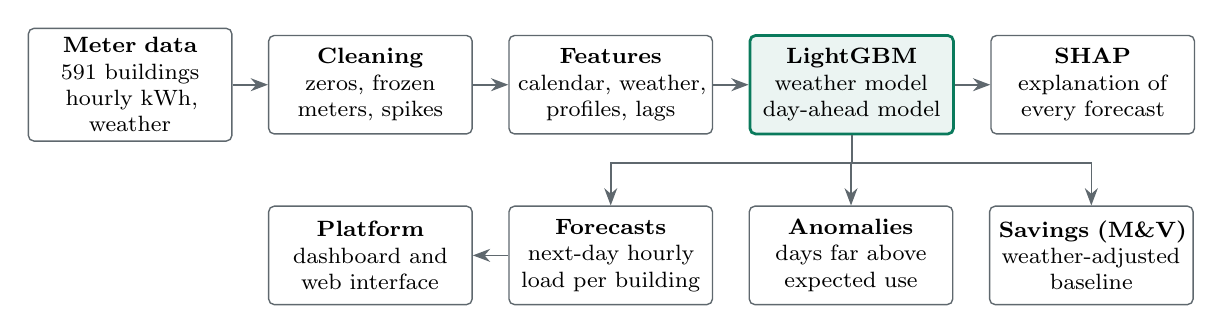
\begin{tikzpicture}[
  node distance=0.55cm and 0.45cm,
  box/.style={draw=ink!70, line width=0.5pt, rounded corners=2pt, align=center, font=\footnotesize,
              minimum height=1.25cm, text width=2.35cm, fill=white},
  key/.style={box, draw=bacai, line width=1pt, fill=bacai!8},
  arr/.style={-{Stealth[length=2.2mm]}, line width=0.6pt, draw=ink!70}]
\node[box] (data) {\textbf{Meter data}\\591 buildings\\hourly kWh, weather};
\node[box, right=of data] (clean) {\textbf{Cleaning}\\zeros, frozen\\meters, spikes};
\node[box, right=of clean] (feat) {\textbf{Features}\\calendar, weather,\\profiles, lags};
\node[key, right=of feat] (models) {\textbf{LightGBM}\\weather model\\day-ahead model};
\node[box, right=of models] (xai) {\textbf{SHAP}\\explanation of\\every forecast};
\node[box, below=0.9cm of feat] (fc) {\textbf{Forecasts}\\next-day hourly\\load per building};
\node[box, right=of fc] (anom) {\textbf{Anomalies}\\days far above\\expected use};
\node[box, right=of anom] (mv) {\textbf{Savings (M\&V)}\\weather-adjusted\\baseline};
\node[box, left=of fc] (app) {\textbf{Platform}\\dashboard and\\web interface};
\draw[arr] (data) -- (clean);
\draw[arr] (clean) -- (feat);
\draw[arr] (feat) -- (models);
\draw[arr] (models) -- (xai);
\draw[arr] (models.south) -- ++(0,-0.35) -| (fc.north);
\draw[arr] (models.south) -- ++(0,-0.35) -| (anom.north);
\draw[arr] (models.south) -- ++(0,-0.35) -| (mv.north);
\draw[arr] (fc) -- (app);
\end{tikzpicture}
\caption{Overview of Baseline AI. Both models share the cleaning and feature pipeline; the weather model supports anomaly
detection and savings verification, the day-ahead model supports operational forecasts. All outputs are explained
with SHAP and exposed in a dashboard and a web platform.}
\label{fig:pipeline}
\end{figure}

\subsection{Problem formulation}
Let $y_{b,t}$ be the electricity use of building $b$ in hour $t$. We learn a function $f$ that maps a feature
vector $\mathbf{x}_{b,t}$ to $\log(1+y_{b,t})$ and predict $\hat{y}_{b,t} = \exp\!\big(f(\mathbf{x}_{b,t})\big)-1$.
Working on the logarithm makes errors relative, so that a hospital and a small office weigh comparably in training,
and stabilises the strongly skewed distribution of loads. One global model is trained for all buildings.

We consider two tasks that differ only in the information available:
\begin{itemize}[leftmargin=1.4em]
  \item \textbf{Weather model} (expected use). $\mathbf{x}_{b,t}$ contains the building identity and type, the site,
        calendar and weather variables and the building's historical profiles, but no recent meter readings.
        Its prediction is the consumption that weather and calendar explain, which is the quantity anomaly
        detection and M\&V require: a fault or a retrofit must not leak into the benchmark.
  \item \textbf{Day-ahead model} (operational forecast). $\mathbf{x}_{b,t}$ also contains loads observed at least
        24 hours before $t$, i.e.\ information available when a forecast for the next day is issued at midnight.
\end{itemize}

\subsection{Features}
Table~\ref{tab:features} lists the features. Building profiles act as target encodings: they are averages of
$\log(1+y)$ computed on the training period only. The \emph{recent} profiles cover the last eight weeks of training
and capture slow drifts in a building's level. Lagged features use only data at least 24 hours old.

\begin{table}[ht]
\centering
\caption{Features. The weather model uses the first four groups; the day-ahead model uses all five.}
\label{tab:features}
\small
\begin{tabularx}{\linewidth}{@{}l X@{}}
\toprule
Group & Features \\
\midrule
Identity & building identifier, site, building type (categorical) \\
Calendar & hour of day, day of week, month, hour of week, weekend flag, public-holiday flag \\
Weather & temperature, relative humidity, dew point (Magnus formula), cooling and heating degree hours
          (base 18\,$^\circ$C), 24\,h and 72\,h mean temperature, temperature 3\,h earlier, daily maximum and minimum \\
Building profile & mean $\log$-load; mean by hour of week; mean by month; recent mean and recent mean by hour
          of week (last 8 weeks of training) \\
Lagged load & load 24\,h, 48\,h, 168\,h and 336\,h earlier; mean of the previous day; mean of the previous week \\
\bottomrule
\end{tabularx}
\end{table}

\subsection{Models}
We compare five approaches.
\textbf{Weekly-profile baseline:} the building's training-period mean for the same hour of the week.
\textbf{Last-week baseline} (day-ahead task): the load of the same hour one week earlier.
\textbf{Ridge regression} on standardised numerical features and one-hot building types ($\alpha=1$).
\textbf{Random forest} \citep{breiman2001random} with 60 trees, maximum depth 24, minimum leaf size 5 and 60\% of
features per split, trained on a random sample of 600\,000 training rows for tractability.
\textbf{LightGBM} \citep{ke2017lightgbm} with squared loss on $\log(1+y)$, learning rate 0.05, 63 leaves, minimum
leaf size 500, feature fraction 0.85, bagging fraction 0.8 and $\ell_2$ regularisation 1, with building, site and
type as native categorical features. We also report an ensemble of the LightGBM and random-forest weather models
(weights 0.7 and 0.3).

\subsection{Validation protocol}
All models are trained on 1 January 2016 to 30 June 2017 (6.64 million rows) and tested on 1 July to 31 December
2017 (2.60 million rows). No test data is used for training, feature construction or any modelling decision.
Feature sets, hyper-parameters and the number of boosting rounds are chosen on a \emph{validation} period, May--June
2017, using models trained on data before May 2017 \emph{and building profiles recomputed from that earlier data
only}. This last point matters: in a first version, profiles that included the validation months made the
validation error optimistic and stopped boosting after about 45 rounds. The number of rounds selected on the
leak-free validation period (175 for the weather model, 214 for the day-ahead model) is increased by 10\% for the
final fit on the full training period.

\subsection{Metrics}
For each building, with $n$ test hours, observed loads $y_i$, predictions $\hat{y}_i$ and mean $\bar{y}$:
\begin{equation}
\cvrmse = \frac{100}{\bar{y}}\sqrt{\frac{1}{n}\sum_{i=1}^{n}(y_i-\hat{y}_i)^2},\qquad
\nmbe = \frac{100}{n\,\bar{y}}\sum_{i=1}^{n}(y_i-\hat{y}_i).
\end{equation}
These are the goodness-of-fit measures of M\&V practice, where hourly models are commonly accepted when
$\cvrmse\le 30\%$ and $|\nmbe|\le 10\%$ \citep{ashrae2014guideline14}. We report the median over buildings, the share of
buildings meeting both limits, and, over all test hours, the root mean squared logarithmic error (RMSLE) and the mean
absolute error (MAE).

\subsection{Explainability}
For each LightGBM model we compute exact TreeSHAP values \citep{lundberg2020trees} on 20\,000 random test hours, in
units of $\log(1+y)$, and summarise feature importance by the mean absolute SHAP value.

\subsection{Anomaly detection}
Detection works on daily totals. For building $b$ and day $d$, let $A_d$ be the metered energy and $E_d$ the sum of
the weather model's hourly predictions. Because buildings drift over months, the expectation is re-calibrated with
the ratio of metered to expected energy over 28 days ending 7 days before $d$,
\begin{equation}
c_d = \frac{\sum_{k=d-34}^{d-7} A_k}{\sum_{k=d-34}^{d-7} E_k},\qquad
r_d = \frac{A_d - c_d E_d}{c_d E_d}.
\end{equation}
The seven-day gap prevents an ongoing fault from raising its own expectation. A day is flagged when
\begin{equation}
r_d > \max\!\Big(0.15,\; \operatorname{med}_b(r) + 2.5 \times 1.4826\,\operatorname{MAD}_b(r)\Big),
\end{equation}
that is, when consumption is at least 15\% above expectation and an outlier for that building according to the
robust median absolute deviation \citep{leys2013mad}. Consecutive flagged days form an event, ranked by excess
energy in kWh.

To measure detection performance we inject synthetic faults into real test data: in 100 randomly chosen buildings,
consumption is multiplied by 1.3 (or 1.5) during five consecutive days at a random date, and we record the share of
fault days flagged and the share of other days flagged in the same buildings.

\subsection{Savings verification}
Following the adjusted-baseline approach of M\&V protocols \citep{evo2022ipmvp,granderson2016accuracy}, a retrofit at
date $t_r$ is evaluated by training the weather model on all data before $t_r$ (with profiles recomputed up to
$t_r$) and predicting the post-retrofit baseline $\hat{B}_t$. The estimated saving over the reporting period is
\begin{equation}
\hat{S} = 1-\frac{\sum_{t\ge t_r} A_t}{\sum_{t\ge t_r}\hat{B}_t}.
\end{equation}
We validate this with $t_r =$ 1 October 2017 and a three-month reporting period. We apply a known saving of 15\% to
the metered data after $t_r$ and measure the error $\hat{S}-0.15$ in each building. We also run a placebo test
without any saving, where the ideal estimate is zero.

%------------------------------------------------------------------ 5
\section{Results}\label{sec:results}

\subsection{Model selection on the validation period}
Table~\ref{tab:tuning} shows the variants compared on May--June 2017. Smaller, more regularised trees with the
recent-profile features were best for both tasks. Removing the day-of-year feature alone did not help, but it was
kept out of the final models because, with only 18 months of history, it allows a model to memorise specific
dates. The test period played no role in these choices.

\begin{table}[ht]
\centering
\caption{Variants compared on the validation period (May--June 2017). ``Original'' trees: 255 leaves, minimum leaf
size 100, learning rate 0.08; ``smaller'' trees: 63 leaves, minimum leaf size 500, learning rate 0.05.}
\label{tab:tuning}
\footnotesize\setlength{\tabcolsep}{4pt}
\begin{tabular}{llrrr}
\toprule
Task & Variant & Rounds & Median CV-RMSE (\%) & Median $|$NMBE$|$ (\%) \\
\midrule
Weather   & original features and trees                   &  45 & 22.12 & 8.80 \\
          & + recent profiles                              &  49 & 21.84 & 8.47 \\
          & + recent profiles, no day of year              &  40 & 22.54 & 9.29 \\
          & + recent, no day of year, smaller trees & 175 & \textbf{21.49} & \textbf{7.95} \\
\midrule
Day-ahead & original features and trees                   &  46 & 15.46 & 3.12 \\
          & + recent profiles, no day of year              &  45 & 15.65 & 3.39 \\
          & + recent, no day of year, smaller trees & 214 & \textbf{14.95} & \textbf{2.18} \\
\bottomrule
\end{tabular}
\end{table}

\subsection{Accuracy on unseen months}
Table~\ref{tab:main} and Figure~\ref{fig:comparison} report test-period accuracy. For the day-ahead task, LightGBM
reduces the median CV-RMSE from 22.95\% for the last-week baseline to 13.76\%, a 40\% reduction, and raises the share of
buildings within the hourly accuracy limits from 73\% to 88\%. For the weather task, LightGBM improves on the
weekly-profile baseline from 28.4\% to 21.5\% and on ridge regression (24.9\%); it is comparable to the random
forest (21.8\%), and the ensemble of the two brings a marginal further gain (21.3\%). The bias of all weather models
(median $|$NMBE$|$ around 6.5\%) is larger than that of the day-ahead model (1.3\%), which shows that much of the
remaining error comes from slow changes in buildings that weather and calendar cannot explain.

\begin{table}[ht]
\centering
\caption{Test-period accuracy (1 July -- 31 December 2017, 591 buildings). CV-RMSE, NMBE and the share within
limits are computed per building; RMSLE and MAE over all test hours. Best value per task in bold.}
\label{tab:main}
\footnotesize\setlength{\tabcolsep}{4.5pt}
\begin{tabular}{llrrrrr}
\toprule
Task & Model & \multicolumn{1}{c}{Median} & \multicolumn{1}{c}{Median} & RMSLE & MAE & Within \\
     &       & \multicolumn{1}{c}{CV-RMSE (\%)} & \multicolumn{1}{c}{$|$NMBE$|$ (\%)} & & (kWh) & limits (\%) \\
\midrule
Weather   & Weekly-profile baseline     & 28.38 & 8.63 & 0.421 & 24.45 & 44.3 \\
          & Ridge regression            & 24.87 & 7.63 & 0.447 & 25.66 & 51.6 \\
          & Random forest               & 21.77 & 6.67 & 0.432 & 23.34 & 57.9 \\
          & LightGBM                    & 21.49 & \textbf{6.43} & \textbf{0.425} & 22.86 & \textbf{58.9} \\
          & Ensemble LightGBM + RF      & \textbf{21.30} & 6.51 & 0.426 & \textbf{22.79} & 58.5 \\
\midrule
Day-ahead & Same hour last week         & 22.95 & \textbf{1.19} & 0.324 & 15.22 & 72.8 \\
          & LightGBM                    & \textbf{13.76} & 1.29 & \textbf{0.206} & \textbf{10.60} & \textbf{88.2} \\
\bottomrule
\end{tabular}
\end{table}

\begin{figure}[ht]
\centering
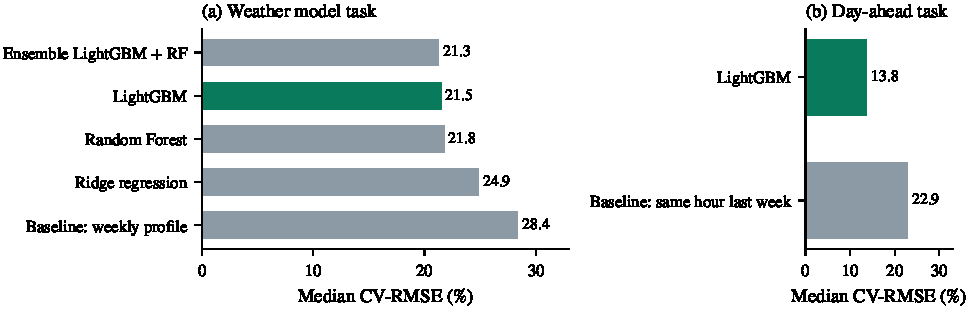
\includegraphics[width=\linewidth]{figures/model_comparison.pdf}
\caption{Median CV-RMSE on the test period. LightGBM models in green.}
\label{fig:comparison}
\end{figure}

Figure~\ref{fig:distribution} shows the distribution over buildings. For the day-ahead model, the CV-RMSE has
quartiles of 9.9\%, 13.8\% and 19.6\%, and 90\% of buildings stay below 29.6\%. The weather model has quartiles of
14.7\%, 21.5\% and 33.1\%, with a long tail of buildings whose consumption changed abruptly after the training
period. Figure~\ref{fig:weeks} shows two weeks for the median building of three common types: both models follow the
daily and weekly cycles, and the day-ahead model also tracks changes of level.

\begin{figure}[ht]
\centering
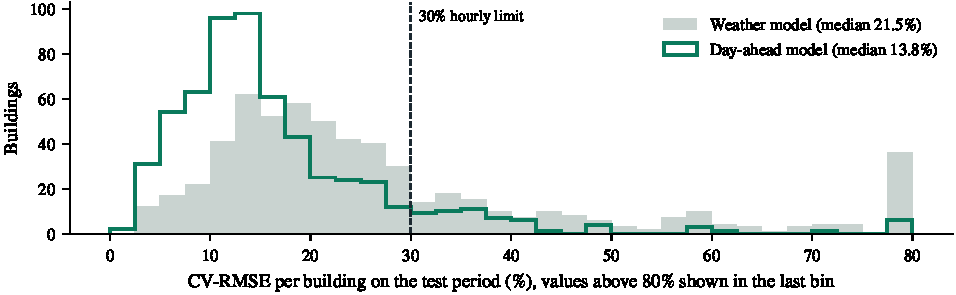
\includegraphics[width=\linewidth]{figures/error_distribution.pdf}
\caption{Distribution of per-building CV-RMSE on the test period. Dashed line: 30\% hourly limit.}
\label{fig:distribution}
\end{figure}

\begin{figure}[ht]
\centering
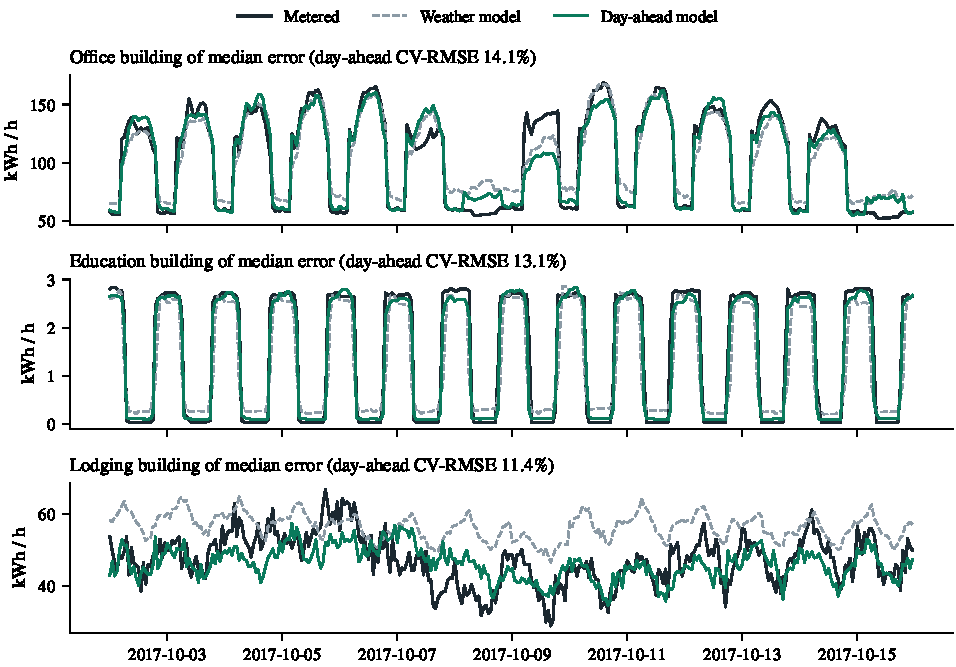
\includegraphics[width=\linewidth]{figures/example_weeks.pdf}
\caption{Metered load and predictions for 2--15 October 2017, for the building of median day-ahead error among
offices, education and lodging buildings.}
\label{fig:weeks}
\end{figure}

Table~\ref{tab:types} breaks the error down by building type. Lodging, parking and education buildings, whose
occupancy follows regular schedules, are the easiest to predict. Assembly, retail and warehouse buildings, whose use
depends on events and operations not visible in the features, are the hardest.

\begin{table}[ht]
\centering
\caption{Median CV-RMSE (\%) by building type, test period. Types with at least seven buildings.}
\label{tab:types}
\small
\begin{tabular}{lrrr}
\toprule
Building type & Buildings & Weather model & Day-ahead model \\
\midrule
Education & 243 & 20.1 & 13.1 \\
Public    &  94 & 19.4 & 14.1 \\
Assembly  &  78 & 33.2 & 17.7 \\
Office    &  70 & 21.5 & 13.8 \\
Lodging   &  52 & 19.5 & 11.4 \\
Parking   &  15 & 14.4 &  7.8 \\
Other     &   9 & 19.7 & 13.2 \\
Retail    &   8 & 29.9 & 20.4 \\
Health    &   7 & 21.4 & 14.1 \\
Warehouse &   7 & 57.7 & 20.8 \\
\bottomrule
\end{tabular}
\end{table}

\subsection{Explanations}
Figure~\ref{fig:shap} ranks features by mean absolute SHAP value. The weather model relies first on the building's
weekly and monthly profiles, then on its identity, mean level and outdoor temperature. The day-ahead model relies
first on the load 24 hours earlier, then on the weekly profile and the loads one week and 48 hours earlier.
Figure~\ref{fig:temperature} isolates the contribution of temperature and dew point in the weather model: it is
lowest around 15--20\,$^\circ$C and rises steeply above roughly 25\,$^\circ$C, the cooling signature expected on
these campuses; it also rises, more mildly, at low temperatures, consistent with some electric heating. The models
therefore use physically plausible drivers.

\begin{figure}[ht]
\centering
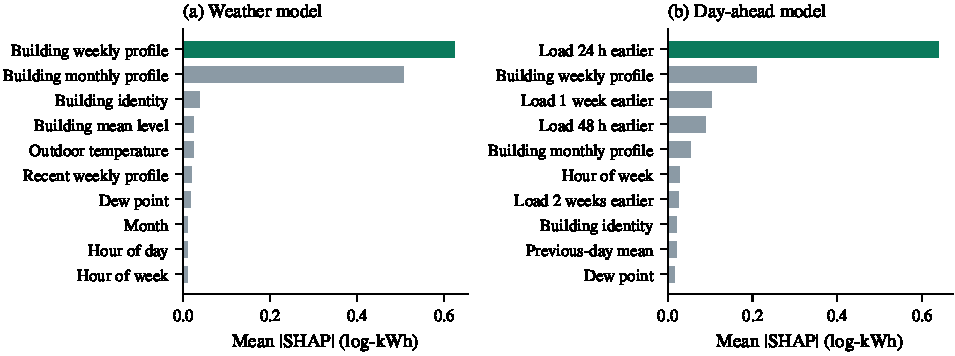
\includegraphics[width=\linewidth]{figures/shap_importance.pdf}
\caption{Top ten features by mean absolute SHAP value (20\,000 test hours, log-kWh units).}
\label{fig:shap}
\end{figure}

\begin{figure}[ht]
\centering
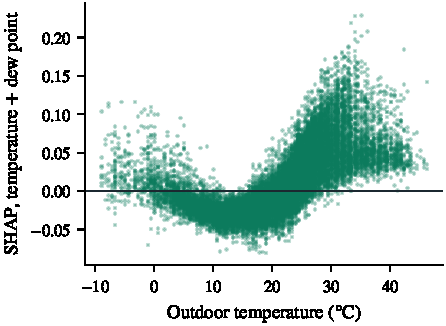
\includegraphics[width=0.52\linewidth]{figures/temperature_effect.pdf}
\caption{SHAP contribution of temperature and dew point in the weather model as a function of outdoor temperature.}
\label{fig:temperature}
\end{figure}

\subsection{Anomaly detection}
On the test period, the detector flags 4\,038 building-days (3.7\% of days), grouped into 1\,600 events, most of them
lasting one or two days. Figure~\ref{fig:anomaly} shows a multi-day event in one building. In the fault-injection
experiment (Table~\ref{tab:apps}), 74.2\% of days with a +50\% fault and 54.6\% of days with a +30\% fault are
detected, while 3.4--3.6\% of normal days are flagged, about one day per month per building. The rolling
calibration matters: without it, the same detector caught 50.6\% of +30\% fault days and flagged 3.2\% of normal days.

\begin{figure}[ht]
\centering
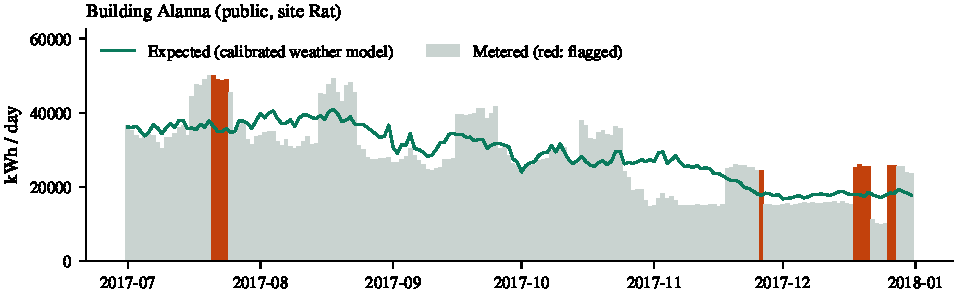
\includegraphics[width=\linewidth]{figures/anomaly_example.pdf}
\caption{Daily metered and expected energy for one building over the test period; flagged days in red.}
\label{fig:anomaly}
\end{figure}

\begin{table}[ht]
\centering
\caption{Validation of the applications on real test data.}
\label{tab:apps}
\small
\begin{tabularx}{\linewidth}{@{}l X r@{}}
\toprule
Experiment & Setting & Result \\
\midrule
Fault detection & +50\% for 5 days, 100 buildings & 74.2\% of fault days flagged \\
Fault detection & +30\% for 5 days, 100 buildings & 54.6\% of fault days flagged \\
False alarms    & normal days in the same buildings & 3.4--3.6\% flagged \\
Savings (M\&V)  & 15\% saving after 1 Oct.\ 2017, 3 months, 591 buildings & median error 6.7 points \\
                &                                    & 42.5\% within 5 points \\
                &                                    & 64.8\% within 10 points \\
Placebo         & no saving applied                   & median estimate $-1.6\%$ \\
\bottomrule
\end{tabularx}
\end{table}

\subsection{Savings verification}
With the baseline retrained up to the retrofit date, the estimated saving has a median absolute error of 6.7
percentage points against a true 15\% saving, 42.5\% of buildings are within 5 points and 64.8\% within 10 points
(Figure~\ref{fig:mv}). The placebo estimates are centred close to zero (median $-1.6\%$), so the method is nearly
unbiased across the portfolio. A simpler variant that only rescaled the original weather model with one calibration
factor gave a median error of 7.6 points and a placebo median of $-3.1\%$. At the level of single buildings and
three months of data, the uncertainty is therefore of the order of the savings of light retrofits; the method is
reliable for large savings, for portfolios, or with longer reporting periods.

\begin{figure}[ht]
\centering
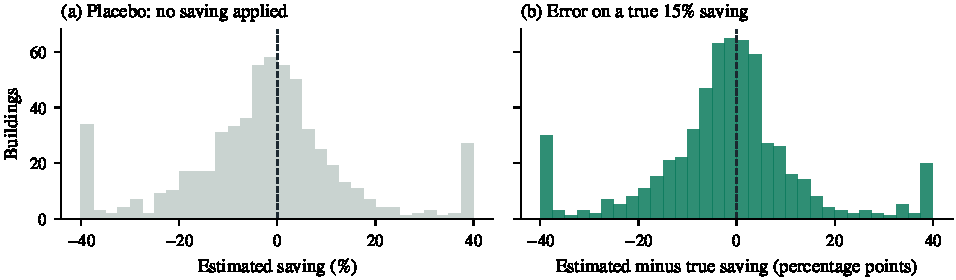
\includegraphics[width=\linewidth]{figures/mv_errors.pdf}
\caption{Savings verification over three months for 591 buildings. (a) Estimated saving when nothing changed.
(b) Error of the estimate when a true 15\% saving is applied. Values beyond $\pm$40 are shown at the edges.}
\label{fig:mv}
\end{figure}

\subsection{Computational cost}
The complete training script (features for the validation and test protocols, two baselines, ridge, random forest
and both LightGBM models, predictions for 9.2 million rows and evaluation) runs in 9.3 minutes on a 4-core CPU with
15\,GB of memory. The full pipeline, including data download, explanations and validation experiments, runs in about
30 minutes. No GPU is needed.

%------------------------------------------------------------------ 6
\section{Discussion}\label{sec:discussion}

\textbf{Impact.} The results support three uses. For facility teams, a daily comparison with the calibrated weather
model surfaces large waste events within days, with about one false alarm per building per month. For utilities and
operators, day-ahead forecasts within the usual accuracy limits for 88\% of buildings can be aggregated into campus
or feeder load and support demand response. For efficiency programmes and their funders, the retrained baseline
gives a nearly unbiased, weather-adjusted estimate of savings across a portfolio. Because one global model covers
all buildings and needs only meter and weather data, the cost of adding a building is negligible, in contrast with
per-building engineering simulation.

\textbf{What limits accuracy.} The gap between the weather model (21.5\%) and the day-ahead model (13.8\%) is mostly
bias: buildings change over months in ways that weather and calendar do not explain (new equipment, occupancy,
operating schedules). Recent-profile features and rolling calibration reduce, but do not remove, this effect.

\textbf{Limitations.} (i) Weather is limited to temperature and humidity; solar radiation and cloud cover are not
available in this distribution of the data. (ii) Floor area and occupancy are not used. (iii) Faults in the detection
experiment are synthetic step changes; real faults, such as gradual degradation or schedule errors, may be easier or
harder to detect, and labelled fault data from facility teams would give a stronger test. (iv) The rolling calibration
adapts to a fault that lasts several weeks: after the seven-day gap, a long fault raises its own expectation and is
no longer flagged, so long-lasting excess must be tracked with a fixed reference period. (v) The buildings are
university campuses in four locations; results may differ for other climates and building stocks. (vi) Deep
sequence models \citep{hochreiter1997lstm,lim2021tft} were not evaluated in this study.

%------------------------------------------------------------------ 7
\section{Software and platform}
Baseline AI is implemented in Python with pandas, scikit-learn \citep{pedregosa2011scikit}, LightGBM and SHAP. One
command downloads the data and runs cleaning, training, explanation and validation; a separate importer prepares
any hourly meter file with the columns \texttt{timestamp}, \texttt{building\_id}, \texttt{kwh},
\texttt{temperature} and \texttt{humidity}. A Streamlit dashboard shows forecasts, anomalies, SHAP explanations and a
savings calculator for every building, and a web platform presents the results for representative buildings in the
browser at \url{https://baselineai.bacai.space}. The code is available at
\url{https://github.com/ouahab4/baseline-ai}.

%------------------------------------------------------------------ 8
\section{Conclusion}\label{sec:conclusion}
Baseline AI shows that a single, explainable gradient-boosting system trained on meter and weather data can forecast the
hourly electricity use of hundreds of real buildings within standard accuracy limits, and can turn these forecasts
into validated tools for waste detection and savings verification. On six unseen months, the day-ahead model reduces
the error of a seasonal baseline by 40\%, and the weather model provides an unbiased benchmark of expected use at the
portfolio level. Future work at COMPILIX INNOVATIONS will add solar radiation and occupancy proxies, probabilistic
(quantile) forecasts, transfer learning to buildings with short histories, comparison with deep sequence models, and
control strategies that use the forecasts for demand flexibility.

\section*{Data availability}
The meter and weather data are from the open Building Data Genome 2 dataset \citep{miller2020bdg2}, released under
the CC BY 4.0 licence, accessed through the BuildingsBench distribution \citep{emami2023buildingsbench}. All
results in this paper are produced by the released code.

\section*{Acknowledgements}
The author thanks the creators and maintainers of the open datasets used in this work.

%------------------------------------------------------------------ references
\small
\begin{thebibliography}{99}\setlength{\itemsep}{0.15em}

\bibitem[Amasyali and El-Gohary(2018)]{amasyali2018review}
K.~Amasyali and N.~M. El-Gohary.
\newblock A review of data-driven building energy consumption prediction studies.
\newblock \emph{Renewable and Sustainable Energy Reviews}, 81:1192--1205, 2018.

\bibitem[ASHRAE(2014)]{ashrae2014guideline14}
ASHRAE.
\newblock \emph{Guideline 14-2014: Measurement of Energy, Demand, and Water Savings}.
\newblock Atlanta, GA, 2014.

\bibitem[Breiman(2001)]{breiman2001random}
L.~Breiman.
\newblock Random forests.
\newblock \emph{Machine Learning}, 45(1):5--32, 2001.

\bibitem[Crawley et~al.(2001)]{crawley2001energyplus}
D.~B. Crawley, L.~K. Lawrie, F.~C. Winkelmann, W.~F. Buhl, Y.~J. Huang, C.~O. Pedersen, R.~K. Strand, R.~J. Liesen,
D.~E. Fisher, M.~J. Witte, and J.~Glazer.
\newblock EnergyPlus: creating a new-generation building energy simulation program.
\newblock \emph{Energy and Buildings}, 33(4):319--331, 2001.

\bibitem[Emami et~al.(2023)]{emami2023buildingsbench}
P.~Emami, A.~Sahu, and P.~Graf.
\newblock BuildingsBench: A large-scale dataset of 900K buildings and benchmark for short-term load forecasting.
\newblock In \emph{Advances in Neural Information Processing Systems 36, Datasets and Benchmarks Track}, 2023.

\bibitem[EVO(2022)]{evo2022ipmvp}
Efficiency Valuation Organization.
\newblock \emph{International Performance Measurement and Verification Protocol: Core Concepts}.
\newblock 2022.

\bibitem[Granderson et~al.(2016)]{granderson2016accuracy}
J.~Granderson, S.~Touzani, C.~Custodio, M.~D. Sohn, D.~Jump, and S.~Fernandes.
\newblock Accuracy of automated measurement and verification (M\&V) techniques for energy savings in commercial
buildings.
\newblock \emph{Applied Energy}, 173:296--308, 2016.

\bibitem[Hochreiter and Schmidhuber(1997)]{hochreiter1997lstm}
S.~Hochreiter and J.~Schmidhuber.
\newblock Long short-term memory.
\newblock \emph{Neural Computation}, 9(8):1735--1780, 1997.

\bibitem[Ke et~al.(2017)]{ke2017lightgbm}
G.~Ke, Q.~Meng, T.~Finley, T.~Wang, W.~Chen, W.~Ma, Q.~Ye, and T.-Y. Liu.
\newblock LightGBM: A highly efficient gradient boosting decision tree.
\newblock In \emph{Advances in Neural Information Processing Systems 30}, pages 3146--3154, 2017.

\bibitem[Leys et~al.(2013)]{leys2013mad}
C.~Leys, C.~Ley, O.~Klein, P.~Bernard, and L.~Licata.
\newblock Detecting outliers: Do not use standard deviation around the mean, use absolute deviation around the
median.
\newblock \emph{Journal of Experimental Social Psychology}, 49(4):764--766, 2013.

\bibitem[Lim et~al.(2021)]{lim2021tft}
B.~Lim, S.~{\"O}. Ar{\i}k, N.~Loeff, and T.~Pfister.
\newblock Temporal Fusion Transformers for interpretable multi-horizon time series forecasting.
\newblock \emph{International Journal of Forecasting}, 37(4):1748--1764, 2021.

\bibitem[Lundberg and Lee(2017)]{lundberg2017unified}
S.~M. Lundberg and S.-I. Lee.
\newblock A unified approach to interpreting model predictions.
\newblock In \emph{Advances in Neural Information Processing Systems 30}, 2017.

\bibitem[Lundberg et~al.(2020)]{lundberg2020trees}
S.~M. Lundberg, G.~Erion, H.~Chen, A.~DeGrave, J.~M. Prutkin, B.~Nair, R.~Katz, J.~Himmelfarb, N.~Bansal, and
S.-I. Lee.
\newblock From local explanations to global understanding with explainable AI for trees.
\newblock \emph{Nature Machine Intelligence}, 2(1):56--67, 2020.

\bibitem[Miller et~al.(2020a)]{miller2020bdg2}
C.~Miller, A.~Kathirgamanathan, B.~Picchetti, P.~Arjunan, J.~Y. Park, Z.~Nagy, P.~Raftery, B.~W. Hobson, Z.~Shi, and
F.~Meggers.
\newblock The Building Data Genome Project 2, energy meter data from the ASHRAE Great Energy Predictor III
competition.
\newblock \emph{Scientific Data}, 7:368, 2020.

\bibitem[Miller et~al.(2020b)]{miller2020gepiii}
C.~Miller, P.~Arjunan, A.~Kathirgamanathan, C.~Fu, J.~Roth, J.~Y. Park, C.~Balbach, K.~Gowri, Z.~Nagy, A.~D.
Fontanini, and J.~Haberl.
\newblock The ASHRAE Great Energy Predictor III competition: Overview and results.
\newblock \emph{Science and Technology for the Built Environment}, 26(10):1427--1447, 2020.

\bibitem[Pedregosa et~al.(2011)]{pedregosa2011scikit}
F.~Pedregosa, G.~Varoquaux, A.~Gramfort, V.~Michel, B.~Thirion, O.~Grisel, M.~Blondel, P.~Prettenhofer, R.~Weiss,
V.~Dubourg, J.~Vanderplas, A.~Passos, D.~Cournapeau, M.~Brucher, M.~Perrot, and {\'E}.~Duchesnay.
\newblock Scikit-learn: Machine learning in Python.
\newblock \emph{Journal of Machine Learning Research}, 12:2825--2830, 2011.

\end{thebibliography}

\end{document}
